\documentclass[11pt,a4paper,oldfontcommands]{memoir}
\usepackage[utf8]{inputenc}
\usepackage[T1]{fontenc}
\usepackage{microtype}
\usepackage[dvips]{graphicx}
\usepackage{subcaption}
\setlength{\parindent}{1em}
\setlength{\parskip}{0.8em}

\usepackage[
breaklinks=true,colorlinks=true,
%linkcolor=blue,urlcolor=blue,citecolor=blue,% PDF VIEW
linkcolor=black,urlcolor=black,citecolor=black,% PRINT
bookmarks=true,bookmarksopenlevel=2]{hyperref}

\usepackage{geometry}
% PDF VIEW
% \geometry{total={210mm,297mm},
% left=25mm,right=25mm,%
% bindingoffset=0mm, top=25mm,bottom=25mm}
% PRINT
\geometry{total={210mm,297mm},
left=20mm,right=20mm,
bindingoffset=10mm, top=25mm,bottom=25mm}

\OnehalfSpacing
%\linespread{1.3}

%%% CHAPTER'S STYLE
\chapterstyle{bianchi}
%\chapterstyle{ger}
%\chapterstyle{madsen}
%\chapterstyle{ell}
%%% STYLE OF SECTIONS, SUBSECTIONS, AND SUBSUBSECTIONS
\setsecheadstyle{\Large\bfseries\sffamily\raggedright}
\setsubsecheadstyle{\large\bfseries\sffamily\raggedright}
\setsubsubsecheadstyle{\bfseries\sffamily\raggedright}


%%% STYLE OF PAGES NUMBERING
%\pagestyle{companion}\nouppercaseheads 
%\pagestyle{headings}
%\pagestyle{Ruled}
\pagestyle{plain}
\makepagestyle{plain}
\makeevenfoot{plain}{\thepage}{}{}
\makeoddfoot{plain}{}{}{\thepage}
\makeevenhead{plain}{}{}{}
\makeoddhead{plain}{}{}{}


\maxsecnumdepth{subsection} % chapters, sections, and subsections are numbered
\maxtocdepth{subsection} % chapters, sections, and subsections are in the Table of Contents






%MOJE USTAWIENIA-------------------------------------------------------------------------

\usepackage[polish]{babel}
\usepackage{listings}
\renewcommand{\lstlistingname}{Kod}
\usepackage{color}
\usepackage[colorinlistoftodos]{todonotes}
\usepackage{amsthm}
\usepackage{longtable}
\usepackage{pdflscape}
\usepackage{graphicx}
\usepackage{color, colortbl}
\usepackage{pgfplots}
\usepackage{subcaption}
\usepackage{url}
\usepackage[resetlabels,labeled]{multibib}
\usepackage{framed}
\usepackage{lipsum}
\usepackage{amsmath}

\usepackage{amsthm}
\usepackage{enumerate}
\usepackage{mathrsfs}
\usepackage[normalem]{ulem}
\usepackage{float}

\usepackage{caption}


\captionsetup[table]{name=Tabela}

\theoremstyle{plain}
\newtheorem{theorem}{Theorem}[chapter]
\newtheorem{prop}[theorem]{Proposition}
\newtheorem{corollary}[theorem]{Corollary}
\newtheorem{lemma}[theorem]{Lemma}


\theoremstyle{definition}
\newtheorem{defn}[theorem]{Definicja}
\newtheorem{ex}[theorem]{Przykład}
\newtheorem{exer}[theorem]{Ćwiczenie}
\newtheorem{refer}[theorem]{Reflection}

\theoremstyle{remark}
\newtheorem{remark}[theorem]{Remark}
\newtheorem{note}[theorem]{Note}
\newtheorem{caut}[theorem]{CAUTION}

% set the default code style
\lstset{
    frame=tb, % draw a frame at the top and bottom of the code block
    tabsize=4, % tab space width
    showstringspaces=false, % don't mark spaces in strings
    numbers=left, % display line numbers on the left
    commentstyle=\color{green}, % comment color
    keywordstyle=\color{blue}, % keyword color
    stringstyle=\color{darkred} % string color
}



\definecolor{dkgreen}{rgb}{0,0.6,0}
\definecolor{gray}{HTML}{d9d9d9}
\definecolor{mauve}{HTML}{ffe6e6}

\newcites{New}{The other list}
\lstset{frame=tb,
  language=Java,
  aboveskip=3mm,
  belowskip=3mm,
  showstringspaces=false,
  columns=flexible,
  basicstyle={\small\ttfamily},
  numbers=none,
  numberstyle=\tiny\color{gray},
  keywordstyle=\color{blue},
  commentstyle=\color{dkgreen},
  stringstyle=\color{red},
  breaklines=true,
  breakatwhitespace=true,
  tabsize=3,
}
% for placeholder text
\usepackage{lipsum}


\newtheorem{mydef}{Definition}


\renewcommand\appendixtocname{Dodatki}
\renewcommand\appendixpagename{Dodatki}

\renewcommand\lstlistingname{Listing}
\renewcommand\lstlistlistingname{Spis pseudokodów}

 \newcommand{\AR}[1]{\todo[inline, color=blue!30]{AR: #1}}
 \newcommand{\MM}[1]{\todo[inline, color=green!30]{MM: #1}}

\newcommand{\HRule}{\rule{\linewidth}{0.5mm}} % Defines a new command for the horizontal lines, change thickness here 

 
\begin{document}

%\begin{titlepage}

\begin{center} % Center everything on the page
 
%----------------------------------------------------------------------------------------
%	HEADING SECTIONS
%----------------------------------------------------------------------------------------

\textsc{\LARGE Politechnika Wrocławska}\\[1.5cm] % Name of your university/college
\textsc{\Large Wydział Elektroniki}\\[0.5cm] % Major heading such as course name
%\textsc{\large ...}\\[0.5cm] % Minor heading such as course title

%----------------------------------------------------------------------------------------
%	TITLE SECTION
%----------------------------------------------------------------------------------------

\HRule \\[0.4cm]
{ \huge \bfseries Testowanie mutacyjne -- optymalizacja procesu i~praktyczne zastosowania}\\[0.4cm] % Title of your document
\HRule \\[1cm]

\textsc{\large \textbf{Rozprawa doktorska }}
\\[1.5cm]
 
%----------------------------------------------------------------------------------------
%	AUTHOR SECTION
%----------------------------------------------------------------------------------------

\begin{minipage}{0.4\textwidth}
\begin{flushleft} \large
\emph{Autor:}\\
mgr Michał Mnich 
\end{flushleft}
\end{minipage}
~
\begin{minipage}{0.4\textwidth}
\begin{flushright} \large
\emph{Promotor:} \\
dr hab. Adam Roman
\end{flushright}
\end{minipage}\\[2cm]

% If you don't want a supervisor, uncomment the two lines below and remove the section above
%\Large \emph{Author:}\\
%John \textsc{Smith}\\[3cm] % Your name

%----------------------------------------------------------------------------------------
%	DATE SECTION
%----------------------------------------------------------------------------------------

\includegraphics[scale=1]{OpisSystemu_IMG/pwr_logo.jpg}\\[1cm] % Include a department/university logo - this will require the graphicx package

{\large \today}\\[2cm] % Date, change the \today to a set date if you want to be precise

%----------------------------------------------------------------------------------------
%	LOGO SECTION
%----------------------------------------------------------------------------------------


 
%----------------------------------------------------------------------------------------

\vfill % Fill the rest of the page with whitespace
\end{center}

%\end{titlepage}

%%%---%%%---%%%---%%%---%%%---%%%---%%%---%%%---%%%---%%%---%%%---%%%---%%%
%%%---%%%---%%%---%%%---%%%---%%%---%%%---%%%---%%%---%%%---%%%---%%%---%%%




%%%---%%%---%%%---%%%---%%%---%%%---%%%---%%%---%%%---%%%---%%%---%%%---%%%
%%%---%%%---%%%---%%%---%%%---%%%---%%%---%%%---%%%---%%%---%%%---%%%---%%%
\newpage
Podziękowania 

\newpage

\tableofcontents*
 
 \newpage
\listoffigures
 
 \newpage
\listoftables

\newpage
\lstlistoflistings

\clearpage
%%%---%%%---%%%---%%%---%%%---%%%---%%%---%%%---%%%---%%%---%%%---%%%---%%%
%%%---%%%---%%%---%%%---%%%---%%%---%%%---%%%---%%%---%%%---%%%---%%%---%%%

\chapter{Wstęp}
\markboth{Wstęp}{Wstęp}
\section{Cel pracy}
lorem ipsum

\section{Tezy badawcze} \label{sec:tezy}

lorem ipsum:
\begin{itemize}
\item[Teza 1.] lorem ipsum

\item[Teza 5.]lorem ipsum
\end{itemize}


\section{Struktura pracy}
Rozdziały WhatisTestingChapter, sec:mutation, section:mutOpt są rozdziałami wstępnymi. Zawierają rys historyczny, przegląd najnowszych badań, modele teoretyczne związane z inżynierią oprogramowania i testowaniem mutacyjnym oraz inne znane z literatury metody optymalizacji testowania. Kolejne rozdziały (section:MutInOneCeompilation, section:MutationChurnMode, section:bayes, TDDM:chapter) prezentują oryginalne wyniki autora pracy. Rozdział framework opisuje architekturę platformy do testów mutacyjnych wykonanej na potrzeby badań zawartych w tej rozprawie. Ostatni rozdział (Summary:chapter) jest rozdziałem zawierającym podsumowanie pracy. Szczegółowa zawartość rozdziałów wygląda następująco:

\begin{itemize}
\item Rozdział WhatisTestingChapter zawiera rys historyczny i przegląd literatury dotyczącej testowania oprogramowania. Wskazuje na konieczność stosowania coraz to nowszych technik testowania programowania.

\item Rozdział sec:mutation zawiera rys historyczny i przegląd literatury dotyczącej specyficznego obszaru testowania oprogramowania, jakim jest testowanie mutacyjne. 

\item Rozdział section:mutOpt opisuje znane w literaturze podejścia do optymalizacji procesu testowania mutacyjnego, a także krótki przegląd propozycji modeli optymalizacyjnych, które zostały zdefiniowane w rozdziałach późniejszych. 

\item Rozdział section:MutInOneCeompilation zawiera oryginalne rozważania opisujące warunki, w jakich niektóre operatory mutacyjne mogą lub nie mogą współistnieć w jednym kodzie. Na tej podstawie został opracowany model teoretyczny wraz z jego implementacją, realizujący proces testowania mutacyjnego oparty o generację wielu mutantów w jednej kompilacji.

\item W rozdziale section:MutationChurnMode wprowadzono model optymalizacyjny (tzw. 'Mutation Churn Model'), którego celem jest redukcja liczby mutantów w kodzie niepowodująca znaczącego spadku efektywności procesu testowania mutacyjnego. Omówione zostały również wyniki badań empirycznych weryfikujących skuteczność zdefiniowanego modelu.

\item Rozdział section:bayes wprowadza drugi model optymalizacyjny, wykorzystujący techniki probabilistyczne, mianowicie model redukcji liczby mutantów oparty na podejściu bayesowskim. Tak jak w rozdziale poprzednim, również i tu omówiono wyniki badań empirycznych nad skutecznością tego modelu w zastosowaniach praktycznych. 

\item  Rozdział TDDM:chapter zawiera nowatorską propozycję metodyki wytwarzania oprogramowania opartą na mutacyjnym testowaniu oprogramowania. Metodyka ta jest modyfikacją podejścia TDD poprzez wzbogacenie jej o krok analizy mutacyjnej. W rozdziale tym zawarte są wyniki eksperymentów potwierdzających skuteczność zaproponowanego podejścia.

\item  Rozdział framework zawiera opis systemu S.A.M. (Symultanic Automatic Mutation System) — autorskiej aplikacji stworzonej przez autora niniejszej dysertacji. System został zaimplementowany w oparciu o zadany model teoretyczny \cite{WawrzyniakPHD. System S.A.M. jest narzędziem służącym do automatyzowania i zarządzania procesem testowania mutacyjnego. 

\item Rozdział Summary:chapter zawiera wnioski oraz podsumowanie.
\end{itemize}




\chapter{Testowanie oprogramowania \label{WhatisTestingChapter}} 
\markboth{Czym jest testowanie}{Czym jest testowanie}


\chapter{Testowanie mutacyjne\label{sec:mutation}}
\markboth{Testowanie mutacyjne}{Testowanie mutacyjne}
Testowanie mutacyjne jest procesem, którego bezpośrednim celem jest pomiar jakości istniejących testów. Dla zadanego programu generowany jest pewien zbiór modyfikacji kodu. Te modyfikacje nazywa się mutantami.

\section{Mutowanie na bajtkodzie}

sensie jest bardziej rozbudowanym wariantem mechanizmów refleksji, które spotykane są w językach opartych na maszynie wirtualnej\footnote{Maszyna wirtualna kontroluje wszystkie odwołania uruchamianego programu }

Technika manipulacji bajtkodem w celu generacji mutantów stosowana jest między innymi w oprogramowaniu PIT \cite{PIT}, gdzie każdy mutant jest generowany za pomocą frameworka ASM \cite{ASM} służącego do manipulacji kodem w wirtualnej maszynie Javy (JVM). Innym znanym oprogramowaniem stosującym technikę generacji mutantów bezpośrednio na kodzie bajtowym jest oprogramowanie MuJava \cite{Mujava}. Zgodnie z informacjami zawartymi w pracy  Ma, Offutta i Kwona \cite{MuJavadoc} do generowania mutantów na platformie MuJava stosowana jest biblioteka BCEL (Byte Code Engineering Library) \cite{bcel}. 
h \texttt{if} lub \texttt{switch}. Przykład takiego kodu prezentuje listing  \ref{kist:AST}.



\newpage
\begin{lstlisting}[language=C++, caption={Pseudokod opisujący mechanikę optymalizacji polegającej na generowaniu wielu mutantów w jednej kompilacji},label={kist:AST}]
public int eval(int x){
int a = 3, b = 1, y;
y = (M_NO==1)? a + x: // mutant 01
(M_NO==2)? a / x: // mutant 02
(M_NO==3)? a % x: // mutant 03
a * x; // bez mutacji
y += b;
return y;
}
\end{lstlisting}

W powyższym kodzie $M_{NO}$ jest zmienną sterującą oznaczającą mutanta, który ma być uruchomiony. Proces testowania mutacyjnego w tym wypadku przebiega w następujący sposób: 

\begin{lstlisting}[language=C++, caption={Proces testowania mutacyjnego z wieloma mutacjami w kompilacji}]
1. Zdefiniuj M_NO := 1. 
2. Uruchom testy dla mutanta M_NO. 
3. Wygeneruj raport. 
4. M_NO := M_NO + 1. 
5. Jesli M_NO przekracza wartosc liczby mutantow, zakoncz.
6. W przeciwnym razie wroc do kroku 2.
\end{lstlisting}

Powyższa technika została opisana w pracy Kapfhammera, Justa i  Schweiggerta \cite{JustKS2011}.







\chapter{Mutation Churn Model \label{section:MutationChurnMode}}
\markboth{Mutation Churn Model}{Mutation Churn Model}

W tym rozdziale zaproponowany i opisany został model optymalizacji procesu testowania mutacyjnego przewidujący stosowanie analizy mutacyjnej tylko i wyłącznie na zmienionym lub nowym kodzie między wersjami danego oprogramowania. Rozdział zawiera opis założeń modelu optymalizacyjnego, jego praktyczne zastosowanie w eksperymentach oraz podsumowanie uzyskanych wyników potwierdzających poprawność działania modelu. 


\chapter{Podejście bayesowskie do priorytetyzacji mutantów \label{section:bayes}}
\markboth{Bayesowski model optymalizacji}{Bayesowski model optymalizacji}
W każdym projekcie prowadzonym w metodyce z zastosowaniem testowania mutacyjnego możemy zaobserwować propagację mutantów trywialnych (patrz def. \ref{TryvialMutant}) względem projektu. Proces ten polega na tym, że wykryty przez testy w pierwszej iteracji mutant jest także wykrywany w jego następnych iteracjach. Tego typu zjawisko sprawia, że marnowany jest czas oraz moc obliczeniowa na proces generacji i uruchamiania zmutowanego kodu, który nie wnosi żadnej nowej informacji do projektu.

\chapter{TDD+M — metodyka wytwarzania oprogramowania wykorzystująca testowanie mutacyjne \label{TDDM:chapter}}
\markboth{Metodyka TDD+M}{Metodyka TDD+M}

\textit{Badania opisane w poniższym rozdziale zostały opublikowane w Software Quality Journal \cite{MnichRoman}. }  

ści mierzonych parametrów we wszystkich cztery próbach są bliskie rozkładowi normalnemu (wartości $p$ dla testu Shapiro-Wilka dla pokrycia instrukcyjnego: $p$=0.1825 dla grup TDD+M oraz $p=0.02$ dla grup TDD; dla pokrycia mutacyjnego: $p=0.011$ dla grup TDD+M oraz $p=0.01$ dla grup TDD). Możemy zatem zastosować test $F$ aby sprawdzić homogeniczność wariancji w próbkach. W przypadku pokrycia instrukcyjnego $p=0.94$, a w przypadku pokrycia mutacyjnego $p=0.45$, zatem nie możemy odrzucić hipotezy 

\newpage
\begin{table}[!ht]
\centering
\caption{Wyniki testów t-Studenta dla grup TDD+M i TDD\label{tab:StudentTest}}
\begin{tabular}{lrr}
\hline
 & \multicolumn{2}{c}{t-test dla różnicy pomiędzy:} \\ \hline
parametr & pokryciem instrukcyjnym & pokryciem mutacyjnym \\ \hline
$N_{TDD+M}$         & 28 & 28 \\
$N_{TDD}$           & 28 & 28 \\ \hline
średnia TDD+M          & 49.25 & 63.28 \\
średnia TDD            & 31.07 & 39.39\\
średnia różnica     & 18.18 & 23.89 \\ 
95\% przedział ufności & [9.25, 27.10] & [11.93, 35.85]\\ 
sd TDD+M            & 16.77 & 20.63 \\
sd TDD              & 16.54 & 23.90\\ 
SEM TDD+M           & 3.17 & 3.90\\
SEM TDD             & 3.13 & 4.52 \\ \hline
p-value             & 0.0001483 & 0.000191 \\
t-test              & 4.0823 & 4.0048 \\ 
df & 54 & 54 \\ 
błąd std różnicy & 4.45 & 5.97 \\
wielkość efektu (współczynnik $d$ Cohena) & 1.091 & 1.07 \\ \hline
\end{tabular}
\end{table}


\textit{Teza 3.3: jakość zewnętrzna oprogramowania jest wyższa, gdy zamiast TDD stosuje się podejście TDD+M}

Tabela \ref{tab:StudExp02_defects} przedstawia liczbę defektów znalezionych przez suity testowe dla każdej pary (kod, testy).

\begin{table}[H]
\centering
\caption{Defekty znalezione dla każdej pary (kod, testy) \label{tab:StudExp02_defects}}
\begin{tabular}{lrrrrrrrr}
\hline
 & \multicolumn{8}{c}{{Kod z grupy}} \\
Testy z grupy $\downarrow$ & 01M & 02M & 03M & 04M & 05 & 06 & 07 & 08 \\ \hline
01M & -- & -- & -- & -- & -- & -- & -- & -- \\
02M & -- & -- & -- & -- & 11 & -- & --  & -- \\
03M & -- & -- & -- & -- & 18 & -- & -- & -- \\
04M & -- & -- & -- & -- & 11 & -- & -- & -- \\
05  & -- & -- & 5  & -- & -- & -- & -- & -- \\
06  & -- & -- & -- & -- & -- & -- & -- & -- \\
07  & -- & 2  & -- & -- & -- & -- & -- & -- \\
08  & -- & -- & -- & -- & -- & -- & -- & -- \\ \hline
\end{tabular}
\end{table}

Jak widać z tabeli, testy grup TDD+M były w stanie wykryć, średnio, 10 $(=(0+11+18+11)/4)$ defektów w kodzie z grup TDD. Z drugiej strony, testy z grup TDD były w stanie znaleźć, średnio, tylko 1.75 defektu w kodzie z grup TDD+M. Testy z grup 1, 6 i 8 nie były w stanie znaleźć żadnych defektów w żadnym z projektów.












\chapter{System S.A.M. - Symultanic Automatic Mutation System \label{framework}} 
\markboth{System S.A.M.}{System S.A.M.}

lorem ipsum

\subsection{Struktura pokrycia kodu testami w PIT}
Zgodnie z dokumentacją systemu PIT \cite{PIT} pokrycie testami oraz nadawanie pierwszeństwa testom (tzn. priorytetyzacja ich wykonania) opiera się na trzech czynnikach:

\begin{itemize}
\item pokrycie linii,
\item czas wykonania testu,
\item konwencja nazewnictwa testów\footnote{Faworyzowanie testów zawierających nazwę klasy}.
\end{itemize}


\section{Mechanika funkcjonowania systemu S.A.M}

Opis przypadku użycia systemu S.A.M. przedstawiono na rys. \ref{fig:SamUsecase}.
lorem ipsum  \ref{manual}.

\begin{figure}[H]
  \centering
  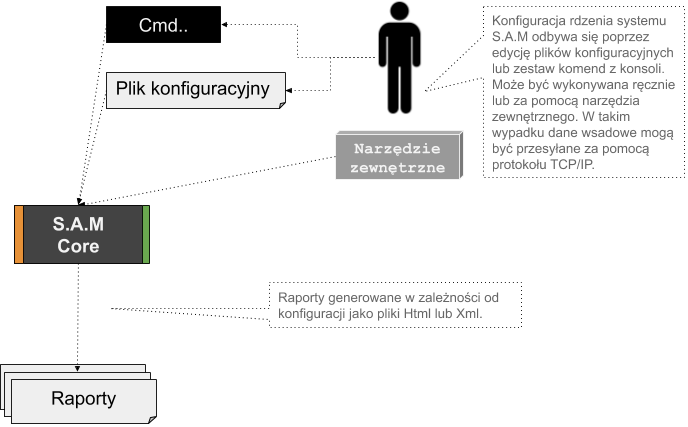
\includegraphics[width=1\textwidth]{OpisSystemu_IMG/UseCase.png}
    \caption{Ogólny opis działania systemu S.A.M.}
   \label{fig:SamUsecase}
 
\end{figure}












\chapter{Wnioski, podsumowanie  \label{Summary:chapter}}

loremIpsum




%BIBLIOGRAFIA----------------------------------------------------

\nocite{*}
\bibliographystyle{unsrt}
\bibliography{bibliography}

%BIBLIOGRAFIA----------------------------------------------------

\begin{appendices}

\chapter{Legenda do tabel \ref{tab:jj412B} oraz \ref{tab:jj412}}
\markboth{Legenda do tabel}{Legenda do tabel}
Poniższa tabela pokazuje nazwy klas wykorzystywanych w eksperymentach w rozdziale 6, gdzie — ze względu na ilość miejsca — kodowane są symbolami c01, c02 itd.


\chapter{Podręcznik systemu generowania wielu mutantów w jednej kompilacji oraz dane dostępowe do repozytorium\label{Appendix:ManualMMIOC}}

\section{Podręcznik}
Niniejszy podręcznik systemu do testowania mutacyjnego oprogramowania korzystającego z technologii generowania wielu mutantów w jednej kompilacji składa się z dwóch sekcji: opisu komend oraz przykładowych uruchomień.

\subsection{Komendy}

\begin{itemize}
\item Program uruchamia się za pomocą komendy \texttt{MMIOC.exe nazwaPlikuCpp}. Przekazywany w parametrze plik ,,cpp'' będzie plikiem, na którym odbędzie się proces mutacji.  

\item \texttt{stat} zwraca statystyki w formie loga oraz CSV. 


\end{itemize}

\subsection{Przykładowe uruchomienia}

Pniżej podana jest pełna sekwencja komend dla pliku \texttt{synt01.cpp}. Plik znajduje się w repozytorium pod adresem:

https://github.com/michaelmnich/-MMIOC/tree/master/MMIOC/CodeSamples/Synthetic

\begin{itemize}
\item Uruchomienie programu: .\textbackslash MMIOC.exe synt01. Uwaga w katalogu .\textbackslash  code\textbackslash musi znajdować się plik synt01.cpp.
\item \texttt{mut -a} -- wygenerowany zostanie w katalogu .\textbackslash code\textbackslash 


\end{itemize}

\section{repozytorium}

Repozytorium projektu znajduje się pod adresem: https://github.com/michaelmnich/-MMIOC



\chapter{S.A.M. — dokumentacja użytkowa oraz dane dostępowe do repozytorium} \label{manual}

LOrem Ipsum \texttt{Java MainWorker}.







\section{Konfiguracja mutacji}
Lorem ipsum \newline



\section{repozytorium}
Repozytoria systemu S.A.M. opisanego w dziale \ref{framework} znajdują się w serwisie Github. 
\begin{itemize}
\item a
\item b
\end{itemize}


\end{appendices}






\end{document}